\documentclass{article}
\usepackage[utf8]{inputenc}
\usepackage{titling} % package per il titolo
\usepackage{graphicx}
\usepackage{hyperref} % package per i collegamenti cliccabili
\usepackage{listings} % package per inserire il codice
\usepackage{xcolor} % package per i colori
\usepackage{float} % usato per le immagini \begin{figure}[H] per mettere la H che evita che le immagini vadano in pagine successive
\usepackage{amsmath}
\usepackage{parskip}
%\usepackage[inner=1cm,outer=1cm,bottom=1cm,top=1cm]{geometry}
\usepackage{geometry}

\title{\Huge Report}
\author{
	\large \textbf{Matteo Battilana} s281389 \\
	\large \textbf{Salvatore Gabriele La Greca} s281589 \\
	\large \textbf{Giovanni Pollo} s290136}
	\date{}
	\renewcommand\maketitlehooka{
		\begin{center}
			
\includegraphics[width=0.8 \textwidth]{Immagini/polito_logo_2021_blu.jpg} % Dimensioni per l'immagine
		\end{center}
		}
		
		\begin{document}
		\begin{titlepage}
			\centering
			\vspace{2px}
		\end{titlepage}
		\maketitle
		\thispagestyle{empty}
		
		\newpage
		
		\thispagestyle{empty}
		
		\section{Explanation}
		
		The idea of the code is to switch cells depending on two priorities in order to reduce leakage power, dynamic power and used area of a combinational circuit. The algorithm is divided into two main different steps, run in order:
		
		\begin{enumerate}
			\itemsep0sp
			\item Swap from LVTs to HVTs: changed accordingly to a certain priority 
			\item Swap performing a gate resizing: changed from a bigger cell to a smaller one based on a priority
		\end{enumerate}
		
		At each change in both the two steps, the slack constraint is checked. If the new slack is lower of the allowed one, the last applied change is reverted.
		
		
		\subsection{Swap from LVTs to HVTs}
		
		The first thing that is executed is the computation of the priority based on the leakage power of each cell. Higher leakage power means higher priority.
		
		The selection of this type of priority is based on previous tests in order to decide the best one. Previous experiments were using priority based on the ratio between the difference of leakage power and difference of delays, between HVT and LVT. We noticed that using a much greedy priority we obtained better results since the computation is much faster.   
		
		Then, after the priority for each cell is defined, the swap can start. In order to avoid useless swaps, only LVT cells are replaced with the corresponding HVT. The swap is done using the PT command \texttt{size\_cell} along with \texttt{update\_timing -full}. The latter command is used in order to avoid mistakes in computation of the new slacks, since it forces a full timing update. 
		
		\subsection{Swap performing a gate resizing}
		After the dual-Vth cell assignment, done in the previous step, the first thing that is executed is the computation of the priority based on area times the dynamic power of each cell. Higher value means higher priority.
		
		\begin{center}
			$P_{areadyn} = Area \cdot P_{dyn}$
		\end{center}
		
		
		Then, after the priority for each cell is defined, the swap can start. This is performed step by steping starting from the original cell size and going lower and lower until new possible swaps are available. The swap is done using the PT command \texttt{size\_cell} along with \texttt{update\_timing -full}. The latter command is used in order to avoid mistakes in computation of the new slacks, since it forces a full timing update. 
		
		\newpage
				\thispagestyle{empty}
		\newgeometry{bottom=1cm}
		\section{Benchmarks}
		\begin{figure}[ht]
			\centering
			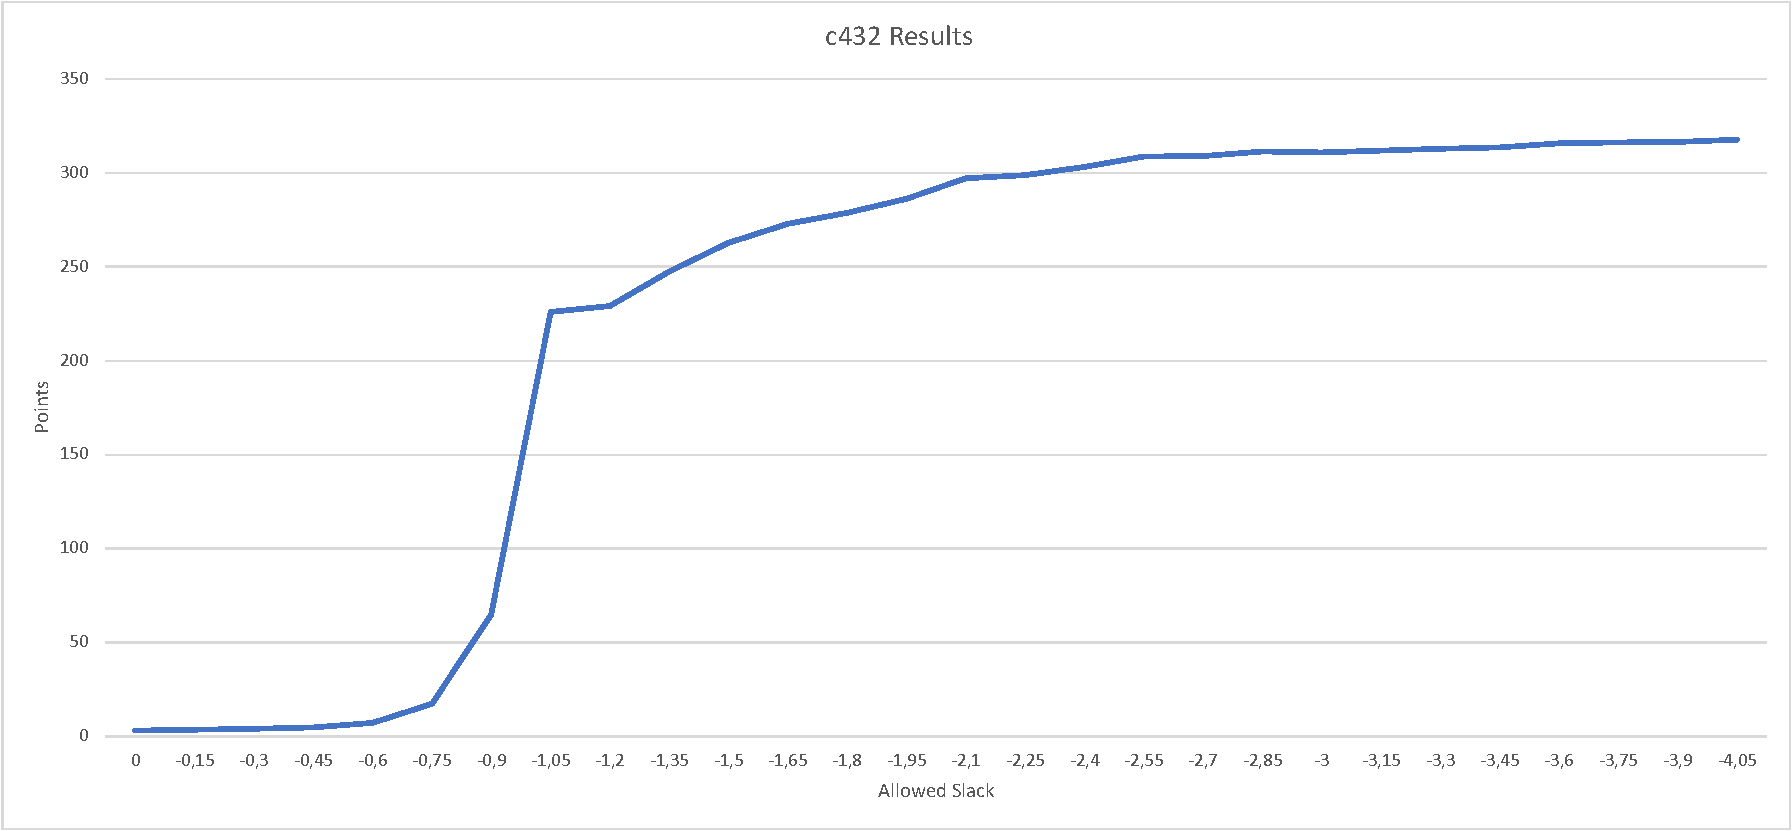
\includegraphics[width=0.6\textwidth]{Immagini/c432.pdf}
		\caption{Results using c432 library}
		\label{benchmark1}
	\end{figure}

	\begin{figure}[ht]
		\centering
		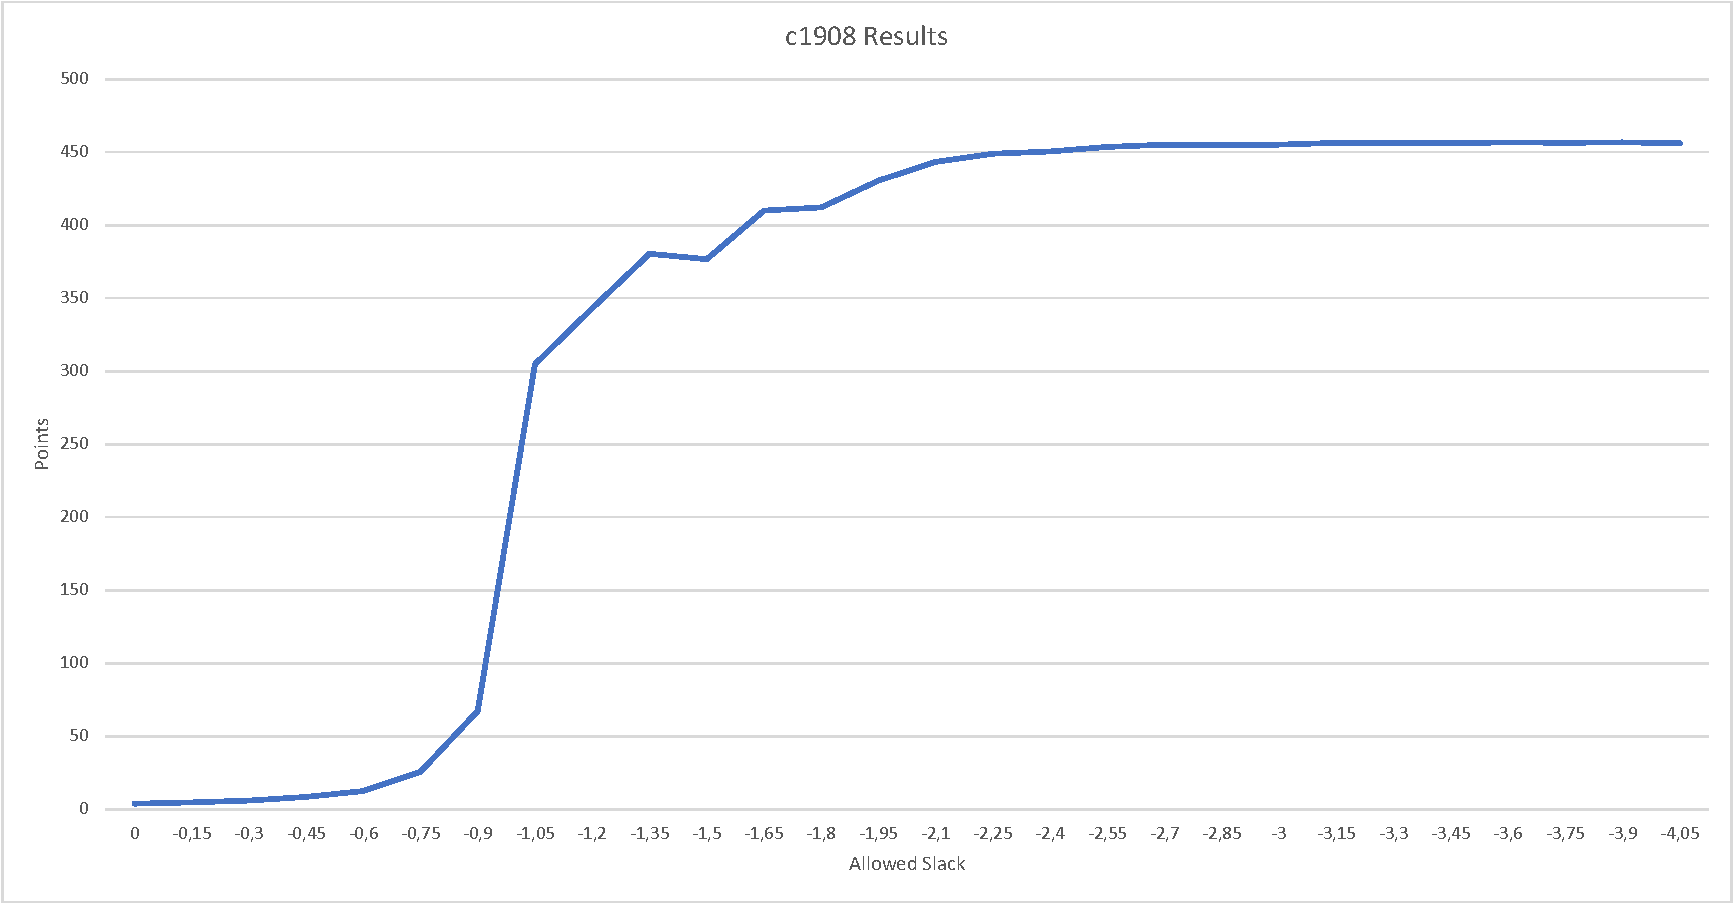
\includegraphics[width=0.6\textwidth]{Immagini/c1908.pdf}
		\caption{Results using c1908 library}
		\label{benchmark2}
	\end{figure}

	\begin{figure}[ht]
		\centering
		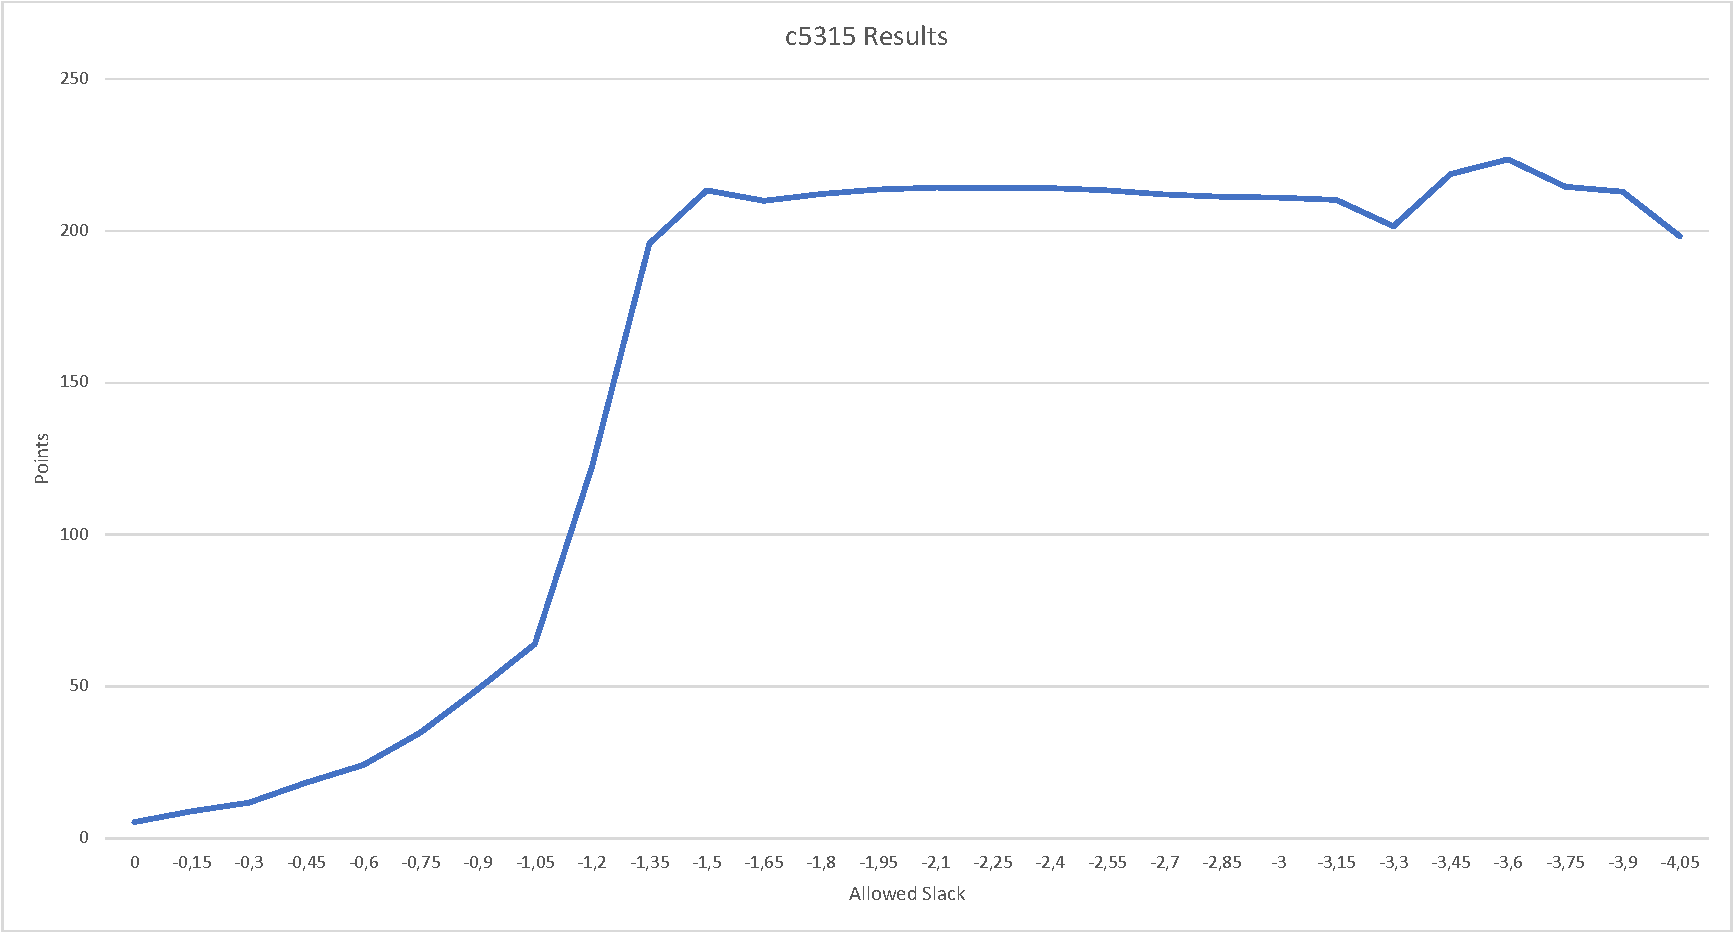
\includegraphics[width=0.6\textwidth]{Immagini/c5315.pdf}
		\caption{Results using c5315 library}
		\label{benchmark3}
	\end{figure}
	
	
\end{document}


